\documentclass[A4paper, 12pt, oneside]{book}
\usepackage[left=1in, right=1in]{geometry}
\usepackage[czech]{babel}
\usepackage{inputenc}
\usepackage[T1]{fontenc}
\usepackage{graphicx}
\usepackage{epstopdf}
\usepackage{setspace}
\usepackage{csquotes}
\usepackage{amsmath, amssymb, amsthm}
\usepackage[inline]{asymptote}
\usepackage{esdiff, icomma, subcaption}
\usepackage{blindtext}

\usepackage[backend=biber, url=true]{biblatex}
\usepackage{url}
\addbibresource{soc.bib}

\newcommand{\B}[1]{\textbf{#1}}
\renewcommand{\S}[1]{\textsc{#1}}
\newcommand{\I}[1]{\textit{#1}}
\newcommand{\mB}[1]{\mathbf{#1}}
\newcommand{\ap}{{\,\prime}}
\newcommand{\abs}[1]{\lvert #1 \,\rvert}

\setstretch{1.3}
\renewcommand*\contentsname{Obsah}
\renewcommand{\theequation}{\arabic{equation}}

\begin{document}
\voffset = -10mm
\begin{center}
	{\LARGE \B{\S{Středoškolská odborná činnost}}} \\
	{\large \B{{Obor č. 2: Fyzika}}}
	\vfill
	{\Huge \B{Mechanika rodin planetek \\ s aplikací na rodinu Eunomia}}
\end{center}
	\vfill
{\large \bfseries Adam Křivka \\
	Jihomoravský kraj \hfill Brno 2018}

\newpage

TODO: Ostatní nutné úvodní stránky pro SOČku...

\newpage
\tableofcontents
\newpage
%\addcontentsline{toc}{section}{Úvod}

\chapter{Úvod do nebeské mechaniky}
TODO: Úvod
\vspace{40mm}
\section{Pohybové rovnice}
Pohybová rovnice je matematicky zapsaný fyzikální vztah, který popisuje možné pohyby těles v daném prostředí \autocite{wiki:eqm}. Řešením pohybové rovnice je funkce, popisující polohu a rychlost každého zkoumaného tělesa v závislosti na čase. Přitom potřebujeme znát počáteční podmínky --- polohy a rychlosti těles na začátku. Pohybová rovnice bývá ve tvaru diferenciální rovnice, což je rovnice, která vyjadřuje vztah mezi nějakou funkcí a jejími derivacemi, což je okamžitá změna hodnoty funkce při velmi malé změně argumentu, v našem případě času. 

V následující části se pokusíme nalézt řešení pohybové rovnice pro tělesa ve sluneční soustavě. Zákony, jimiž se budou naše tělesa řídit, jsou Newtonův gravitační zákon a Newtonovy pohybové zákony, které byly poprvé definovány již v roce 1687.
\subsection{Rovnice pro dvě tělesa}
Omezme se nyní na dvě tělesa a nalezněme řešení tzv. problému dvou těles, někdy také Keplerovy úlohy. To znamená, že se pokusíme odvodit funkci, popisující polohu a rychlost obou těles v závisloti na čase. 

Nacházíme se v inerciální vztažné soustavě, což je taková vztažná soustava, kde platí první Newtonův zákon. Jako bod v klidu si zvolme těžiště soustavy. Pro síly působící na obě tělesa podle Newtonova gravitačního zákona a druhého a třetího pohybového zákona platí
\begin{align} 
	\vec{F}_1 &= +G\frac{m_1m_2}{\abs{\vec{r}}^3}\vec{r} = m_1\vec{a}_1 \label{eq:newton1} \\
	\vec{F}_2 &= -G\frac{m_1m_2}{\abs{\vec{r}}^3}\vec{r} = m_2\vec{a}_2, \label{eq:newton2}
\end{align}
kde $G$ označuje gravitační konstantu, $m_1$, $m_2$ hmotnosti zkoumaných těles, $\vec{a}_1$, $\vec{a}_2$ vektory zrychlení těles (tj. druhé derivace polohových vektorů $\vec{r}_1$, $\vec{r}_2$ podle času) a $\vec{r}$ vektor udávající vzájemnou polohu těles, definovanou jako $\vec{r} = \vec{r}_2 - \vec{r}_1$. Součtem obou rovnic dostáváme
\begin{equation} \label{eq:mr=0}
	\vec{F}_1 + \vec{F}_2 = m_1\vec{a_1} + m_2\vec{a_2} = 0.
\end{equation}
Vektor popisující polohu těžiště soustavy je $\vec{R} \equiv \frac{m_1\vec{r}_1 + m_2\vec{r}_2}{m_1 + m_2}$. Jeho druhou derivací podle času dostáváme zrychlení
\begin{equation*}
	\diff[2]{\vec{R}}{t} = \frac{m_1\vec{a_1} + m_2\vec{a_2}}{m_1+m_2} = 0,
\end{equation*}
které se podle \eqref{eq:mr=0} rovná nule, takže se těžiště soustavy pohybuje konstantní rychlostí.
\newpage
Nyní se však přesuňme do soustavy neinerciální, kde je první z těles (běžně to hmotnější) nehybné. Řekněme, že nehybné těleso má index $1$, tedy nově $\vec{r}^\ap_1=0$, $\vec{r}^\ap_2=\vec{r}$ (tedy i $\vec{a}^\ap_2 = \vec{a}$) a $\vec{r}^\ap=\vec{r}$. Provedli jsme tedy v podstatě transformaci, kdy jsme ke každému vektoru přičetli $\vec{r}_1$.  Rovnici \eqref{eq:newton1} můžeme přepsat jako
\begin{align}
	\nonumber {\vec{a}} = Gm_2\frac{\vec{r}}{\abs{\vec{r}}^3} \\
		\diff[2]{\vec{r}}{t} - Gm_2\frac{\vec{r}}{\abs{\vec{r}}^3} = 0	
\end{align}
Často ještě definujeme gravitační paramter soustavy $\mu=Gm_2$.

I přesto, že tato diferenciální rovnice ještě není ve své konečné podobě vhodné k tomu, abychom z ní vyvodili následující vztah, prozradíme, že je jím funkce v polárních souřadnicích, popisující vzdálenost těles $r\equiv\abs{\vec{r}}$ v závisloti na úhlu $\theta$, který svírá přímka procházející oběma tělesy a nějaká zvolená referenční přímka. 
\begin{equation} \label{eq:polar}
	r(\theta)=\frac{p}{1+e\cos{(\theta-\omega)}}
\end{equation}
kde $p$ se nazývá paramter elipsy, jehož velikost je určena hodnotou $\mu$, $e$, resp. $\omega$ jsou integrační konstanty a nazývají se excentricita, resp. argument pericentra. K rovnici \eqref{eq:polar} a jejím důsledkům se vrátíme v sekci \ref{sec:orbelem}, zatím vězme, že jsme dostali obecnou funkci kuželosečky, z nichž nás bude nejvíce zajímat případ elipsy. Zmíněné konstanty budou určovat její tvar, rozhodně ale nestačí k úplnému popsání orientace trajektorie (orbity) tělesa v prostoru. 

Uvědomme si, že jsme neodvodili závislost polohy tělesa na čase. Tuto závislost určuje Keplerova rovnice:
\begin{equation} \label{eq:kepler}
M = E + e\sin E
\end{equation}
kde $M$ označuje střední anomálii, $E$ excentrickou anomálii a $e$ excentricitu elipsy (viz obrázek). Obě anomálie mají úhlové jednotky, úhel $M$ ale nemůžeme zkonstruovat, nicméně je významný tím, že je lineárně závislý na čase. Pokud známe $E$, můžeme pomocí snadno spočítat $M$.  Problém spočívá v tom, že nemůžeme vyjádřit $E$ v závisloti na $M$ konečným výrazem, ale pouze nekonečnou řadou nebo jej můžeme aproximovat numerickými metodami.

\subsection{Rovnice pro N těles}
Jak vidíme, už i pro dvě tělesa se musíme k získání polohy tělesa v čase uchýlit k numerickým metodám. Ukazuje se, že obecný problém $N$ těles je analyticky neřešitelný\footnote{existují ale nějaká zajímavá speciální řešení, viz \cite{cohan12}.} a jediné aplikovatelné metody jsou metody přibližné analytické nebo numerické.

Uvažujme nyní $N$ těles --- respektive hmotných bodů, které na sebe vzájemně gravitačně působí v souladu s Newtonovým gravitačním zákonem. Pro libovolné těleso, označené indexem $j\in\{1,\,2,\,\dots,\,N\}$, je celková síla $F_j$, která na něj působí, výslednicí všech gravitačních sil způsobených ostatními tělesy, jak ukazuje následující rovnice.
\begin{align} 
	\vec{F}_j = m_j\vec{a}_j &= \sum_{\substack{i=1 \\ i\neq j}}^N G\frac{m_im_j}{\abs{\vec{r}_i-\vec{r}_j}^3}(\vec{r_i}-\vec{r_j}) \label{eq:nbody1}\\
		\vec{a}_j &= \sum_{\substack{i=1 \\ i\neq j}}^N \frac{Gm_i}{\abs{\vec{r}_i-\vec{r}_j}^3}(\vec{r_i}-\vec{r_j}) \label{eq:nbody2}
\end{align}
kde $\vec{r}_i-\vec{r}_j$ označuje vektor určující vzájemnou polohu těles $i$ a $j$, konkrétně jde o vektor s počátkem v tělese $j$ a vrcholem v tělese $i$; ostatní veličiny jsou definované analogicky jako v předchozí části.
\subsubsection{Eulerova metoda}
I přesto, že se následující metoda v přesných numerických výpočtech zřídka používá, uvádíme ji zde z didaktických důvodů, neboť názorně ilustruje použití numerických metod pro řešení problému $N$ těles. Jak název napovídá, poprvé s ní v 18. století přišel švýcarský matematik Leonhard Euler.

Princip algoritmu spočívá v tom, že v libovolném čase můžeme z \eqref{eq:nbody2} vypočítat zrychlení každého tělesa. Pak, po zvolení určitého časového kroku, odpovídajícím způsobem změníme vektor rychlosti. Následně necháme všechna tělesa po dobu časového kroku pohybovat se po přímce konstantní rychlostí. Následuje přesný popis algoritmu a k němu příslušná ilustrace na obrázku \ref{fig:euler}.

Mějme zmiňovaných $N$ hmotných bodů, pro které platí \eqref{eq:nbody2}. Zaměřme se na jeden hmotný bod v čase $t_0$ a označme jeho počáteční polohu $\vec{r}(t_0)$ a počáteční rychlost $\vec{v}(t_0)$. K použití Eulerovy metody potřebujeme znát i počáteční polohy a rychlosti všech ostatních těles v systému. Dále vhodně zvolme velikost časového kroku $h$. V následujícíh třech krocích si ukažéme jednu iterace algoritmu. Pokud bychom chtěli počítat v čase $t_0$, dosadili bychom $k=0$.
\begin{enumerate}
	\item Nechť je v čase $t_k$ poloha zvoleného bodu $\vec{r}(t_k)$ a rychlost $\vec{v}(t_k)$. Z \eqref{eq:nbody2} vypočítáme zrychlení $\vec{a}(t_k)$. 
	\item Položme $t_{k+1} = t_{k}+h$ a vypočítejme $\vec{v}(t_{k+1}) = \vec{v}(t_k) + h\cdot\vec{a}(t_k)$.\footnote{Můžeme porovnat se vzorcem pro rovnoměrný přímočarý pohyb, dobře známým ze středoškolského učiva: $v = v_0 + at$, podobně v kroku 3 $s = s_0 + vt$}
	\item Vypočítejme $\vec{r}(t_{k+1}) = \vec{r}(t_k) + h\cdot\vec{v}(t_k)$ a vraťme se ke kroku 1, tentokrát počítaje v čase $t_{k+1}$. 
\end{enumerate}

\begin{figure}
	\centering
	\begin{asy}
		unitsize(5cm);

		marker mark1 = marker(scale(circlescale*2)*unitcircle, Fill);
		marker mark2 = marker(scale(circlescale*7)*unitcircle, Fill);
		real ascale = 1;
		real vscale = 0.5;

		pair R = (0,0);
		pair r0 = (0.57,-1);
		pair M = 0.3;
		pair m = 1;
		pair G = 1;

		real h = 0.8;

		draw(R, marker=mark2);
		draw(r0, marker=mark1);
		label("$M$", shift(-0.05,-0.05)*R, SW);

		draw(arc(R,length(R-r0), -60, 15), longdashed+gray(0.7));

		// První iterace
		pair a0 = (G*M/(length(R-r0)**2))*unit(R-r0);
		draw(r0--shift(r0)*scale(ascale)*a0, arrow=EndArrow);
		label("$\mathbf{a_0}$", shift(r0)*scale(0.5)*scale(ascale)*a0, SSW);

		pair v0 = rotate(-90)*unit(a0)*sqrt(G*M/(length(R-r0)));
		draw(r0--shift(r0)*scale(vscale)*v0, arrow=EndArrow);
		label("$\mathbf{v_0}$", shift(r0)*scale(0.5)*scale(vscale)*v0, SE);

		pair v1 = v0+h*a0;
		draw(r0--shift(r0)*scale(vscale)*v1, arrow=EndArrow);
		label("$\mathbf{v_1}$", shift(r0)*scale(0.4)*scale(vscale)*v1, NNW); 

		pair r1 = r0 + h*v1;
		draw(r0--r1, dashed);
		draw(r1, marker=mark1);

		// Druhá iterace
		pair a1 = (G*M/(length(R-r1)**2))*unit(R-r1);
		draw(r1--shift(r1)*scale(ascale)*a1, arrow=EndArrow);
		label("$\mathbf{a_1}$", shift(r1)*scale(0.5)*scale(ascale)*a1, SSW);

		// pair v1
		draw(r1--shift(r1)*scale(vscale)*v1, arrow=EndArrow);
		label("$\mathbf{v_1}$", shift(r1)*scale(0.5)*scale(vscale)*v1, SE);

		pair v2 = v1+h*a1;
		draw(r1--shift(r1)*scale(vscale)*v2, arrow=EndArrow);
		label("$\mathbf{v_2}$", shift(r1)*scale(0.4)*scale(vscale)*v2, NW); 

		pair r2 = r1 + h*v2;
		draw(r1--r2, dashed);
		draw(r2, marker=mark1);

		// Třetí iterace
		pair a2 = (G*M/(length(R-r2)**2))*unit(R-r2);
		draw(r2--shift(r2)*scale(ascale)*a2, arrow=EndArrow);
		label("$\mathbf{a_2}$", shift(r2)*scale(0.5)*scale(ascale)*a2, SSW);

		// pair v2
		draw(r2--shift(r2)*scale(vscale)*v2, arrow=EndArrow);
		label("$\mathbf{v_2}$", shift(r2)*scale(0.5)*scale(vscale)*v2, SE);

		pair v3 = v2+h*a2;
		draw(r2--shift(r2)*scale(vscale)*v3, arrow=EndArrow);
		label("$\mathbf{v_3}$", shift(r2)*scale(0.4)*scale(vscale)*v3, NW); 

		pair r3 = r2 + h*v3;
		draw(r2--r3, dashed);
		draw(r3, marker=mark1);

		file fout = output("out.txt");
		write(fout, length(R-r0));
		//write(fout, length(v0));
	\end{asy}
	\caption{Ilustrace Eulerovy metody pro dvě tělesa, kdy větší těleso s pozicí $\vec{R}$ a hmotností $M$ (velká tečka vlevo nahoře) gravitačně působí na menší těleso (malé tečky vpravo). Jsou ukázány iterace $t_0$, kdy vycházíme z počátečních hodnot veličin $\vec{r_0}$ a $\vec{v_0}$, a $t_1$, $t_2$. Algoritmus byl reálně aplikován, se zjednodušenými hodnotami: $h=0,4 \ s$, $M=0,3 \ kg$, $G=1$, $r=R-r_0=1.15 \ m$, $v_0=0,51 \ ms^{-1}$ a obrázek byl mírně upraven pro lepší viditelnost. Šedá křivka naznačuje ideální dráhu tělesa.}
	\label{fig:euler}
\end{figure}

Jak můžeme vidět na obrázku \ref{fig:euler}, vypočtená dráha se od té reálné značně vzdaluje. To by samozřejmě vyřešila volba menší kroku $h$, ale pro velký počet těles a velkou požadovanou přesnost je algoritmus velmi pomalý (tedy konverguje pomalu) a dnešní počítače na něj nestačí.

TODO: O ostatních integračních metodách, udělám až budu víc chápat WHM, RMVS, ... Swift obecně.

\section{Orbitální elementy} \label{sec:orbelem}
TODO: Zavedení šesti základní elementů
\subsection{Oskulační elementy}
TODO: Popis, efemeridy
\subsection{Střední elementy}
\subsection{Vlastní elementy}
TODO: Význam, nastínění výpočtu

\chapter{Planetky ve Sluneční soustavě}
\section{Rodiny planetek}
\subsection{Metody identifikace rodin}
\subsubsection{Rezonance středního pohybu}
\subsubsection{Rezonance sekulární}

\chapter{Vlastnosti rodiny Eunomia}
\begin{figure}
	\centering
	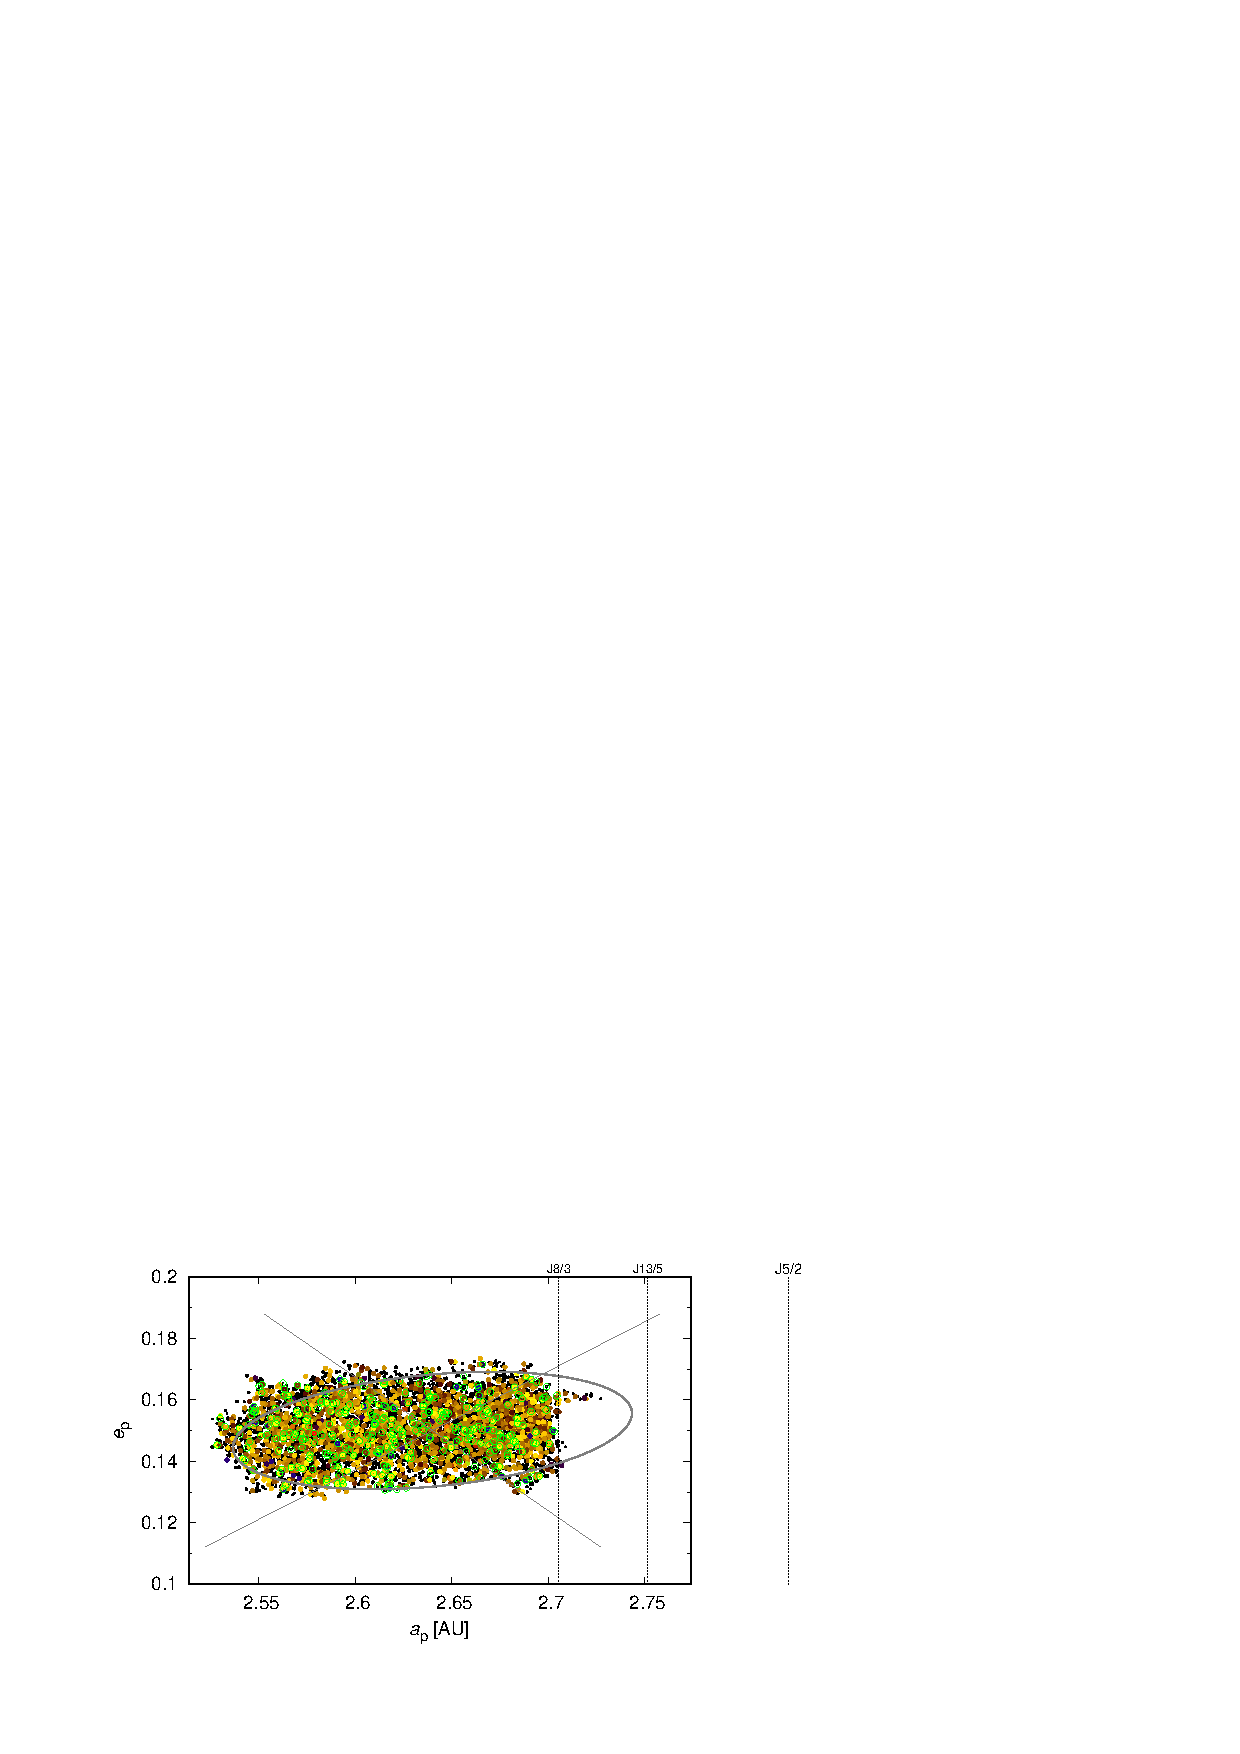
\includegraphics[width=0.5\textwidth]{obr/ae_wise}
	\caption{TODO}
	\label{ae_wise}
\end{figure}
\begin{figure}
	\centering
	\includegraphics[width=0.5\textwidth]{obr/ai_wise}
	\caption{TODO}
	\label{ai_wise}
\end{figure}
\begin{figure}
	\centering
	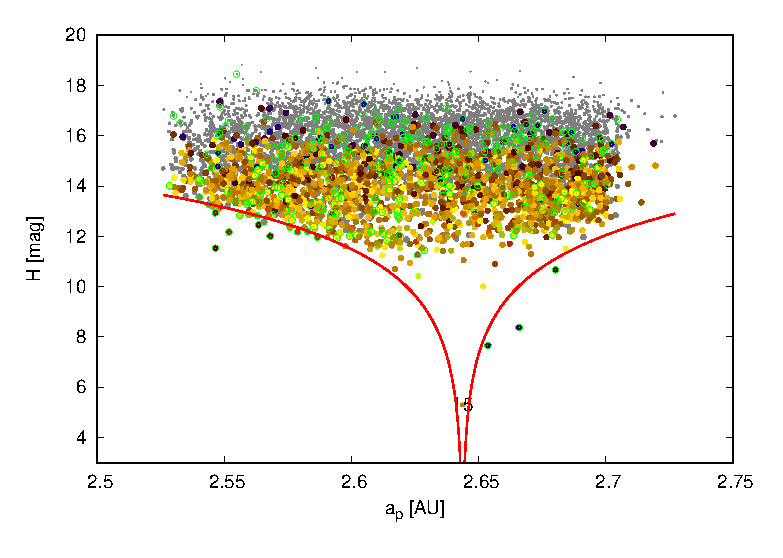
\includegraphics[width=0.5\textwidth]{obr/aH_wise}
	\caption{TODO}
	\label{aH_wise}
\end{figure}
\begin{figure}
	\centering
	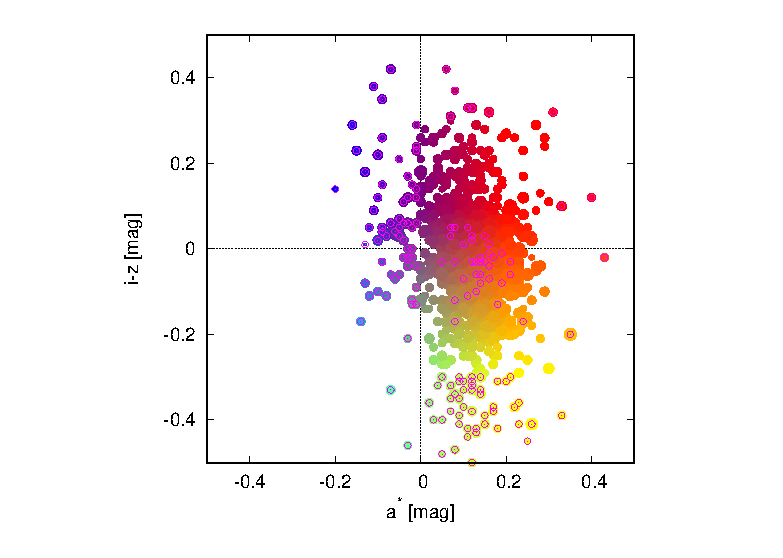
\includegraphics[width=0.5\textwidth]{obr/astar_iz}
	\caption{TODO}
	\label{astar_iz}
\end{figure}
\begin{figure}
	\centering
	\includegraphics[width=0.5\textwidth]{obr/pV_pIR}
	\caption{TODO}
	\label{pV_pIR}
\end{figure}
\begin{figure}
	\centering
	\includegraphics[width=0.5\textwidth]{obr/Nv}
	\caption{TODO}
	\label{Nv}
\end{figure}
\begin{figure}
	\centering
	\begin{subfigure}[b]{0.45\textwidth}
	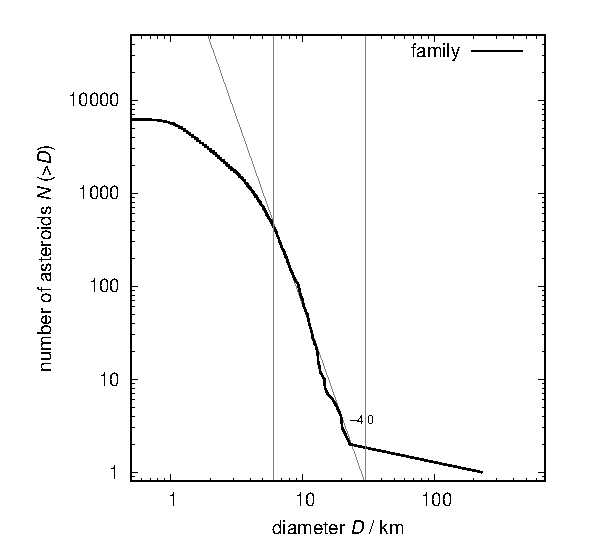
\includegraphics[width=\textwidth]{obr/size_distribution}
	\end{subfigure} ~
	\begin{subfigure}[b]{0.45\textwidth}
	\includegraphics[width=\textwidth]{obr/size_distribution_SMALLD}
	\end{subfigure}
	\caption{TODO}
	\label{size_distribution}
\end{figure}
\section{Nejistoty pozorovaných dat}
\section{Fyzikální model pro rodinu Eunomia}
\subsection{Jarkovského jev}
\subsection{YORP jev}
\subsection{Náhodné srážky}
\subsection{Nevratné děje při vývoji}
\section{Simulace orbitálního vývoje}
\section{Porovnání modelu a pozorování}

\chapter{Aplikace v praxi}
\chapter{Budoucí možnosti výzkumu}
\printbibliography
\end{document}
